%!TEX root = main.tex
\section{Preliminaries: Data and User Models} 
%In this section, we first describe the data model, and the supported visualization types. We then introduce two visualization spaces, and propose a user expectation model to traverse these spaces. Finally, we formally define the problem.

%In this section, we first describe our data model by reporting the visualization and query setup, and corresponding visualization lattice based on data subsets. We then introduce a user expectation model to traverse the lattice and justify its design. Finally, we formally define our problem of finding a collection of informative-and-interesting visualizations from the lattice.

%\subsection{Visualizations and Queries}

\subsection{Data Model}
We assume that we are operating on a dataset consisting of a single relational table R. Our approach also generalizes to multiple tables obeying a star or a snowflake schema, but we focus on the single table case for ease of presentation. 

%\notes{[It seems that the visualization types that can be supported by our framework/system is similar to \textsc{Zenvisage}. In fact, we can use either \textsc{SQL} or \textsc{ZQL} as back-end.]} 

\textbf{Visualization.} We start by defining the notion of a visualization. There are different visualization types such as bar charts, scatter plots, and trend lines, but across all types, a visualization can be defined using five main components: (i) the x-axis attribute(s), (ii) the y-axis attribute, (iii) the subset of data used, (iv) the binning and aggregation functions for the x- and y- axes, and (v) the type of visualization (e.g., bar chart, scatter plot).


\textbf{Query.} \system\ supports visualizations that can be defined in terms of the aforementioned components, covering common visualization types such as bar charts, trend lines, and scatter plots. These visualizations can be translated into the following \textsc{SQL} query: 

\begin{center}
{\tt SELECT X, A(Y) FROM R WHERE C(Z) GROUP BY X}.
\end{center}

Here, $X$ refers to the x-axis attribute(s), $Y$ to the y-axis attribute, $A(Y)$ to the aggregation function on $Y$, $Z$ to the attribute(s) used in specifying the data subset, while $C(Z)$ to the constraint(s) that specify the data subset.

\textbf{Lattice.} Based on the aforementioned notion of visualizations, we conceptualize a visualization lattice based on data subset. 

Given a data subset defined by a set of constraints $C = \{z_1, \ldots, z_n\}$ (on attributes $Z = \{Z_1, ..., Z_n\})$, expanding $C$ by adding one or more new constraints will generate a new data subset that is contained within the former subset. An ancestor-descendant relationship exists between these data subsets. Specifically, a data subset defined by constraints $C_a$ is an ancestor of a data subset defined by constraints $C_b$, if and only if $C_b \subsetneqq C_a$. Further, a data subset defined by constraints $C_a$ is a parent of a data subset defined by constraints $C_b$, if and only if $C_b \subsetneqq C_a \land \mid C_a \mid - \mid C_b \mid = 1$. Notice that, a data subset can have multiple parent subsets. For example, given a sales dataset with four attributes {\tt\{Country, Gender, Month, Price\}}, the data subset defined by constraints {\tt\{Country = US, Month = Jan\}} has two parents--- the data subsets defined by constraints {\tt\{Country = US\}} and {\tt\{Month = Jan\}}.

\begin{figure}[bht]
\label{example}
\centering
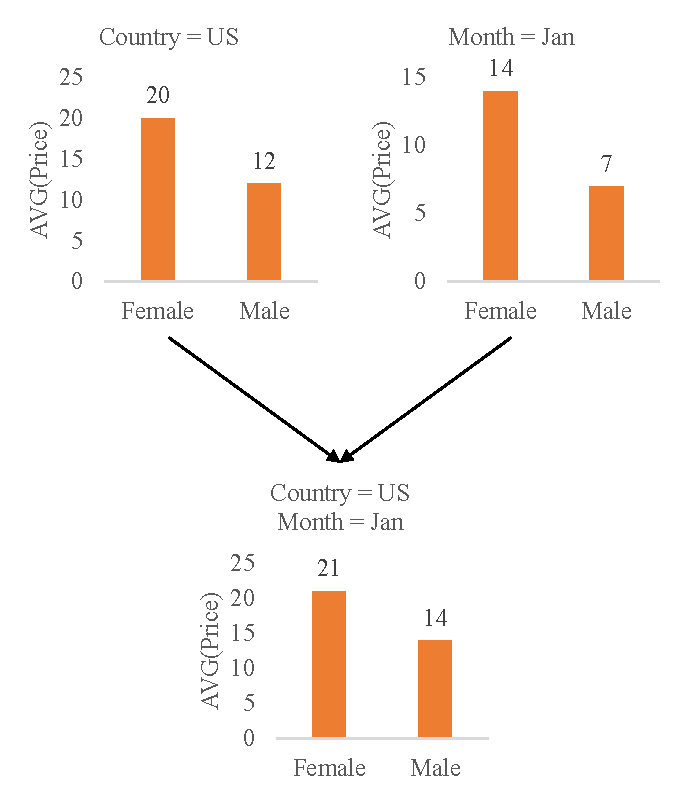
\includegraphics[scale=0.5]{figures/SubsetRelation.pdf}
\caption{Parent Child Relationship in Data Subsets}
\end{figure}

We now extend the concept of parent data subset to introduce the idea of parent visualization. Let $V$ be the set of visualizations (of same type) that show the same $X$ and $Y$ for different $C(Z)$. Given a visualization $V_i \in V$, parent of $V_i$, $V_i^j$ ($V_i^j\in V$) is a visualization that corresponds to a parent data subset of the former. Analogous to a data subset, a visualization $V_i \in V$ can have multiple parents. Figure 1 presents three visualizations that show the average price of products bought by male and female customers for three different data subsets: (i) US citizens, (ii) people who buy products in Jan, (iii) US citizens who buy products in Jan. As per the parent-child relationship between the data subsets, the visualizations corresponding to (i) and (ii) are parents of the visualization corresponding to (iii).

\iffalse
\begin{figure}[bht]
\label{example}
\centering
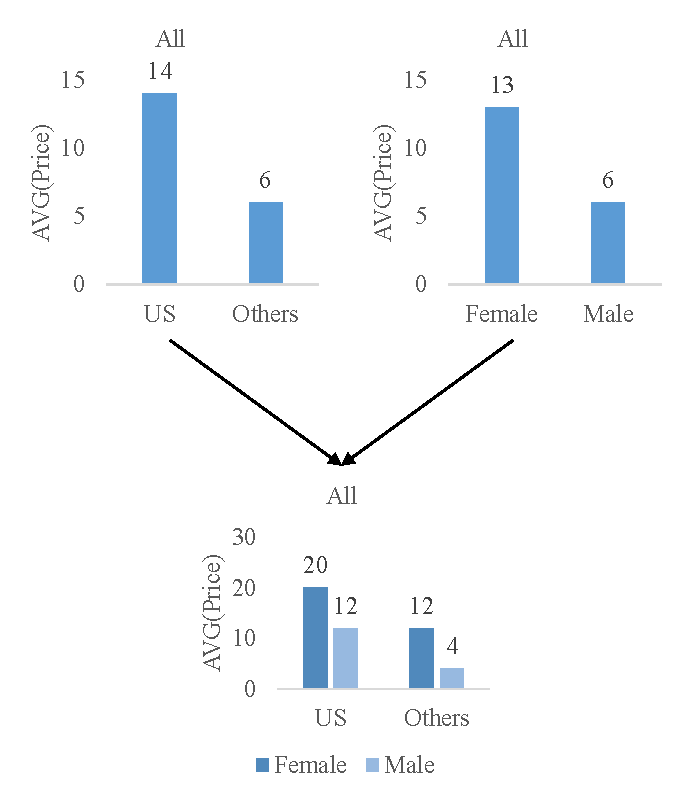
\includegraphics[scale=0.5]{figures/DimensionRelation.pdf}
\caption{Parent Child Relationship in Dimension Combination Space}
\end{figure}

\textbf{Dimension Combination Space.} Given a combination of dimension attributes $X = \{X_1, \ldots, X_n\}$, adding one or more new dimensions in $X$ will generate a new combination.  An ancestor-descendant relationship exists between these dimension combinations. Specifically, a dimension combination $X_a$ is an ancestor of a dimension combination $X_b$, if and only if $X_b \subsetneqq X_a$. Further,  a dimension combination $X_a$ is a parent of a dimension combination $X_b$, if and only if $X_b \subsetneqq X_a \land \mid X_a \mid - \mid X_b \mid = 1$. Notice that, a dimension combination can have multiple parent combinations. For example, given a sales dataset with four attributes {\tt\{Country, Gender, Month, Price\}}, the dimension combination {\tt\{Country, Month\}} has two parent combinations--- {\tt\{Country\}} and {\tt\{Month\}}. 

We now extend the concept of parent dimension combination to introduce the idea of parent visualization. Let $U$ be the set of visualizations (of same type) that show the same $Y$ and $C(Z)$ for different $X$. Given a visualization $V_i \in U$, parent of $V_i$, $V_i^j$ ($V_i^j\in U$) is a visualization that corresponds to a parent dimension combination of the former. Analogous to a dimension combination, a visualization $V_i \in U$ can have multiple parents. Figure 2 presents three visualizations that show the average price of products for three different dimension combinations: (i) US citizens/non-citizens, (ii) males/females, (iii) males/females who are US citizens/non-citizens. As per the parent-child relationship between the dimension combinations, the visualizations corresponding to (i) and (ii) are parents of the visualization corresponding to (iii).
\fi

\subsection{User Expectation Model}
In order to understand which visualizations a user would deem ``informative" and ``interesting" , we consider how analysts explore their data through OLAP operations (drill-down and roll-ups), and model the effective utility of displaying an unseen visualization to a user in the context of other seen visualizations. 

\textbf{Top Down Traversal.} We observe that, while exploring a dataset, users first look at the top level visualizations before looking at the next level. Further, the data distributions learnt from the top level visualizations set user expectation for the next level. Based on these two observations, we model user expectation $\hat{V_i}$ corresponding to an unseen visualization $V_i$ based on its seen/observed parents, $P(V_i) = \{V_i^1, \ldots, V_i^\lambda\}$. Specifically, we model two aspects of each unseen-visualization and observed-parent relationship, namely informativeness and interestingness. 

\textbf{Informativeness.} To model the informativeness of an observed parent in the context of an unseen visualization, we characterize the capability of the parent in predicting the unseen visualization. For an unseen visualization, the observed parents whose data distributions accurately predict the data distribution of the unseen are \emph{informative}. Specifically, we formulate the informativeness of an observed parent $V_i^j$ ($V_i^j \in P(V_i)$) of an unseen visualization $V_i$ as the similarity between their data distributions using a similarity function $S(V_i, V_i^j)$. The most informative parents $V_i^*$ of an unseen visualization $V_i$ are the ones whose data distributions have highest similarity with that of the unseen.

\begin{equation}
    V_i^*=\underset{V_i^j}{argmax}\ S(V_i, V_i^j)
\end{equation}

Since declaring a parent as informative can vary depending on its similarity with the unseen compared to other parents, we allow the user to specify a threshold $\theta$, which we expect to be close to one, such that the similarity score $S(V_i, V_i^{*, \theta})$ corresponding to the informative parents $V_i^{*, \theta}$ are at least $\theta$ fraction of that of the most informative parents'.

\begin{equation}
    V_i^{*, \theta} = \{V_i^j : \frac{S(V_i, V_i^j)}{S(V_i, V_i^*)} \ge \theta\}
\end{equation}

\textbf{Interestingness.} While the informative parents contribute to the prediction of an unseen visualization, the most interesting visualizations to recommend are those for which even the informative parents fail to predict the visualization. To model the interestingness of an unseen visualization $V_i$ in the context of an observed parent $V_i^j$ ($V_i^j \in P(V_i)$), we characterize the deviation between their data distributions using a distance function $D(V_i, V_i^j)$. The unseen visualizations whose data distributions deviate from the observed informative parents are \emph{interesting}. The most interesting unseen visualizations $V_\#$ are the ones that deviate most from their observed informative parents.
\begin{equation}
    V_\#=\underset{V_i}{argmax} \ D(V_i, V_i^{*, \theta})
\end{equation}

%\noindent Additional model extensions can be added to this objective function based user specification. For example, there may be $k$ visualizations that approximately yield equal contribution to the user's expectation. For simplicity of notation, we have assumed $k=1$ in the aforementioned model. In order, a user may want to prevent the recommendation of spuriously interesting subsets of the data. We can discard visualizations that falls below a certain subpopulation size threshold. 

\subsection{Problem Statement}

Given a dataset and user specified x- and y- axes, the goal of our system is to generate a dashboard by selecting $k$ visualizations from the data subset space, where (i) one of the $k$ visualization is the root--- the visualization corresponding to the entire dataset with no constraints, (ii) for each visualization except for the root, at least one of its informative parents is included within the $k$ visualizations, (iii) the $k$ visualizations are collectively most \lq\lq interesting\rq\rq\ in presence of their informative parents, (iv) the number of latent visualizations (not present in dashboard) whose informative parents are present in the dashboard is maximal.

